\chapter{Stavba siete} \label{stavba}

Všetky siete boli napísané v programovacom jazyku \textit{Python} s použitím knižníc \textit{numpy} a \textit{tensorflow}.
Na začiatku bola sieť skonštruovaná so všetkými 44 príznakmi, ktoré sme dostali z transformačnej časti práce (Príloha \ref{in:foot}).
Sieť obsahovala teda vstup o veľkosti 44 príznakov, 2 skryté vrstvy neurónov (s 25, resp. 15 neurónmi) a troj-neurónový výstup typu softmax, ktorý vyberie najpravdepodobnejšiu možnosť, nastaví daný výstup neurónu na 1 a zvyšné nastaví na 0.
Na vylepšovanie siete sme, ako je napísané v jednej z predošlých kapitol (\ref{docu}), použili údaje, ktoré sa napokon budú pri vyhodnocovaní nachádzať medzi testovacími datami. 

V prípade futbalu data prišli v dvoch súboroch, ako trénovacie a finálne vyhodnocovacie, takže sme trénovacie data až v tomto programe rozdelili podobne ako budú rozdelené pri vyhodnocovaní výsledkov. 
Konkrétne, pre futbal data predstavovali 7 celých sezón a prvú polovicu ďalšej sezóny (ako popísané v \ref{foot}), vyhodnocovacie data predstavujú teda druhú polovicu tejto sezóny. 
Takže sme trénovacie data rozdelili na tri časti, 6 celých sezón a polovicu ďalšej (trénovacie data), druhú polovicu siedmej sezóny (trénovacie data) a zvyšnú prvú polovicu ôsmej sezóny (nepoužité data).
V prípade tenisu prišli data už priamo z transformačnej časti v troch súboroch, trénovacie, testovacie a vyhodnocovacie data.

Každá sieť mala svoje nedostatky v celkovej úspešnosti, ale doposiaľ neexistuje efektívne nastavenia neurónových sietí pre každú situáciu \citep{gitgud}, takže každá sieť sa musela vylepšovať osobitne a manuálne vzhľadom na rozdiely v prístupoch.
Cieľom práce nie je porovnať rovnakú architektúru a viac typov neurónových sietí, ale pokúsiť sa získať, čo možno najlepšie výsledky a porovnať potenciály doprednej a rekurentnej neurónovej siete.

\section{Selekcia príznakov}
Kliatba dimenzionality nám hovorí, že čím viac vstupných príznakov zadáme neurónovej sieti, tým sú data redšie a teda je ich potreba získať viac, aby sa sieť správne učila. Viac dat získať nevieme, takže sa pokúsime znížiť počet dimenzií a pozrieť sa na to, ako sa to prejaví na trénovacích datach.
Na začiatok spravíme korelačný test všetkých príznakov testovacích a trénovacích dat (obrázok \ref{corr}).
Teória hovorí, že by nám mohla napovedať, aké hodnoty sú dôležité.
Obrázok hovorí, že najvyššiu koreláciu s výsledkom zápasu majú príznaky 41 a 42 určujúce dlhodobú silu tímu. Skóre dosahuje tiež celkom vysokú koreláciu (okolo 0,2) s finálnym výsledkom.
...

\noindent
\begin{figure} \label{corr}
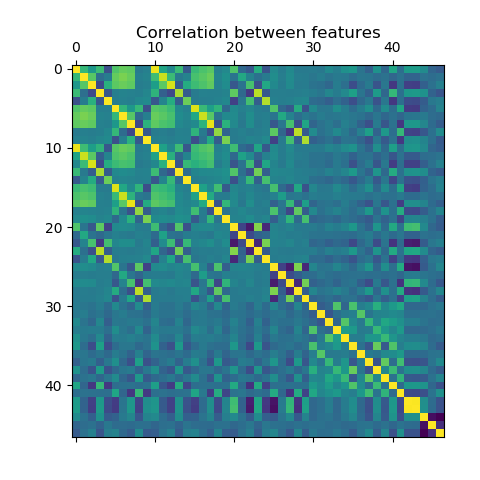
\includegraphics[scale=0.9]{../img/correng.png}
\caption{Korelačná tabuľka všetkých príznakov pre anglickú Premier League, žltá predstavuje kladnú koreláciu, modrá zápornú. Nás hlavne zaujímajú posledné 3 riadku určujúce koreláciu príznaku s výsledkom zápasu (príznaky sú v poradí ako v Prílohe \ref{in:foot}).}
\end{figure}

\iffalse
Pokus 1: bez formy (1-20, 31-44) (ešte práca s dropoutom) 
dropout po 2.(58%, 48%) 9.7. 17:13 epochs 500
dropout po 1. vrstve 9.7. 17:19 54,8% 52,8% epochs 300
Pokus 2: bez GPG -12 stĺpcov
Pokus 3: kombinácia (44-20)
\fi
